\documentclass[a4paper,11pt]{article}


%%% fontenc
%\usepackage{fontspec,xunicode,xltxtra}
%\setmainfont{Times New Roman}
%\setsansfont{Source Sans Pro}
%\setmonofont{Source Sans Pro}

%%% xeCJK
\usepackage{xeCJK}
\setCJKmainfont[BoldFont=Adobe Heiti Std]{Adobe Song Std}
\setCJKsansfont[BoldFont=Adobe Heiti Std]{Adobe Song Std}
\setCJKmonofont[BoldFont=Adobe Heiti Std]{Adobe Song Std}
\XeTeXlinebreaklocale "zh"
\XeTeXlinebreakskip=0pt plus 1pt minus 0.1pt

\usepackage{xcolor}
\usepackage{graphicx}

%%% get total page number
\usepackage{lastpage}

%%% customized definition
\makeatletter
\def\sybtitle#1{\def\@sybtitle{#1}}
\def\sybauthor#1{\def\@sybauthor{#1}}
\def\sybdate#1{\def\@sybdate{#1}}
\sybtitle{}
\sybauthor{}
\sybdate{}
\def\sybmaketitle{
  \begin{center}
  \vspace*{.8in}
  {\huge\bfseries\@sybtitle}
  \par
  \vspace{.8in}
  {\Large\@sybauthor}
  \par
  \vspace{.2in}
  \@sybdate
  \vspace{.5in}
  \end{center}
}
\makeatother
\setlength{\parindent}{0pt}
\renewcommand{\today}{\number\month 月 \number\day 日, ~\number\year 年}
\def\lt{\textless}
\def\gt{\textgreater}
\renewcommand\contentsname{\bfseries 目~~录}
\newcommand\bs{\texttt{\symbol{'134}}} % input backslash sign
%\newcommand\bs{\string\} % same as above definition
\long\def\cmd#1{\par\vspace{.5em}\hspace*{2em}#1\vspace{.5em}\par}
\def\cstr#1{\texttt{\string#1}} % e.g. \cstr{\latex}
\long\def\runcode#1{\par\bigskip#1\bigskip\par}
% 我不想看到那么多的underful hbox,尤其是minted环境加上背景色之后
\hbadness=10000
% 适当放宽overful hbox的限制,运行2pt的溢出
\hfuzz=2pt
\parskip=3\lineskip


%%% change background color & add frame for enumerate enviroment
\usepackage{mdframed}
\newmdenv[backgroundcolor=blue!10,linewidth=0pt]{coloredframe}
\newenvironment{coloredenumerate}{
  \begin{coloredframe}
  \begin{enumerate}
}{
  \end{enumerate}
  \end{coloredframe}
}

%%% geometry
\usepackage[includehead,includefoot,hmargin=21mm,vmargin=10.5mm,
            headsep=12pt,headheight=25pt]{geometry}
%\usepackage[includehead,includefoot,hmargin=1.2in,vmargin=1in]{geometry}

%%% fancyhdr
\usepackage{fancyhdr}
\makeatletter
\fancypagestyle{main} {
  \fancyhf{} % clear header & footer
  \fancyhead[L]{\bfseries\@sybtitle}
  \fancyhead[R]{\thepage/\pageref*{LastPage}}
  \renewcommand{\headrulewidth}{0.4pt} % header line
  \renewcommand{\footrulewidth}{0pt} % footer line
}
\fancypagestyle{header} {
  \fancyhf{} % clear header & footer
  \fancyfoot[C]{\roman{page}}
  \renewcommand{\headrulewidth}{0pt} % header line
  \renewcommand{\footrulewidth}{0pt} % footer line
}
\makeatother

\usepackage{titlesec}
\titleformat{\part}{\centering\Large\bfseries}{第\,\thepart\,部分}{1em}{}
\titleformat{\section}{\large\bfseries}{\thesection}{1em}{}
\titleformat{\subsection}{\normalsize\bfseries}{\thesubsection}{1em}{}
%\titlespacing*{章节命令}{左边距}{上文距}{下文距}[右边距]
\titlespacing*{\section}{0pt}{2\baselineskip}{\parsep}


\usepackage{hyperref}

%%% perfect source code display
\usepackage{minted}
%\usemintedstyle{colorful}
\definecolor{srcbg}{rgb}{0.95,0.95,0.95}
\newminted{java}{linenos,tabsize=4,bgcolor=srcbg}
\newminted{xml}{linenos,tabsize=4,bgcolor=srcbg}
\newminted{cpp}{linenos,tabsize=4,bgcolor=srcbg}
\newminted{bash}{linenos,tabsize=4,bgcolor=srcbg}
\newminted{latex}{linenos,tabsize=4,bgcolor=srcbg}



\usepackage{xcolor}
\colorlet{HEADCOLOR}{red!50}
\colorlet{BRANCHCOLOR}{blue!50}
\colorlet{WORKCOLOR}{gray!50}
\colorlet{INDEXCOLOR}{cyan!50}
\colorlet{COMMITCOLOR}{green}

\usepackage{tikz}
\usetikzlibrary{shapes,arrows,positioning,calc,backgrounds,matrix,fit,decorations.pathreplacing}
\tikzset{
  basic-style/.style = {
    rectangle, rounded corners=2pt, draw, thick,
    fill=#1,
    minimum height=15pt,
    minimum width=1.5cm,
    inner sep=1pt
  },
  commit-style/.style = {
    basic-style=COMMITCOLOR
  },
  index-style/.style = {
    basic-style=INDEXCOLOR,
    minimum width=2.5cm
  },
  work-style/.style = {
    basic-style=WORKCOLOR,
    minimum width=2.5cm
  },
  branch-style/.style = {
    basic-style=BRANCHCOLOR
  },
  head-style/.style = {
    basic-style=HEADCOLOR
  },
  cmd-style/.style = {
    #1=5pt
  },
  cmd-style/.default = right,
  main-style/.style = {
    execute at end picture = {
      \begin{pgfonlayer}{background}
        \path[fill=gray!20,rounded corners]
          ([xshift=-0.2cm,yshift=-0.2cm]current bounding box.south west) rectangle
          ([xshift=0.2cm,yshift=0.2cm]current bounding box.north east);
          %(current bounding box.south west) rectangle
          %  (current bounding box.north east);
        \end{pgfonlayer}
    }
  },
  file-style/.style = {
    draw=red, fill=yellow!30, inner sep=2pt
  },
  dir-style/.style = {
    fill=green!50,inner sep=2pt
  },
  dir-bg-style/.style = {
    fill=cyan!30,rounded corners
  },
  every edge/.style = {draw, ->, >=latex', thick}
}

%%%%% new definitions %%%%%

\newlength\commitDistance
\setlength\commitDistance{0.5cm}
\newlength\indexWorkDistance
\setlength\indexWorkDistance{2\commitDistance}

\newcommand\displayName[1]{\ttfamily\bfseries #1}
\newcommand\commandName[1]{\ttfamily\bfseries\small #1}

\def\createNode style:#1 name:#2 display:#3 direct:#4 distance:#5 to:#6;{
  \node [#1, #4=#5 of #6] (#2) {#3}
        edge [#4] (#6);
}
\def\createCommit name:#1 display:#2 direct:#3 to:#4;{
  \node [commit-style, #3=\commitDistance of #4] (#1) {#2}
        edge [#3, COMMITCOLOR] (#4);
}
\def\createBranch name:#1 display:#2 direct:#3 to:#4;{
  \node [branch-style, #3=0.75\commitDistance of #4] (#1) {#2}
        edge [#3, BRANCHCOLOR] (#4);
}
\def\createHead direct:#1 to:#2;{
  \node [head-style, #1=0cm of #2] (head) {\displayName HEAD};
}
\def\createIndex to:#1;{
  \node [index-style, below=2\commitDistance of #1] (index) {\displayName Index};
}
\def\createWork to:#1;{
  \node [work-style, below=2\commitDistance of #1] (work) {\displayName Work DIR};
}

\newcommand\makeOutline{
  %\useasboundingbox (-0.1,-3.6) rectangle (10.7,2);
  \node[right] (dumy) at (0,0) {\dots};
  \createCommit name:a display:{\displayName A} direct:right to:dumy;
  \createCommit name:b display:{\displayName B} direct:right to:a;
  \createCommit name:c display:{\displayName C} direct:right to:b;
  \createCommit name:d display:{\displayName D} direct:right to:c;
  \createCommit name:e display:{\displayName E} direct:right to:d;

  \createIndex to:c;
  \createWork to:index;
}

\newcommand\createMatrix[2]{
  \matrix [
    matrix of nodes,
    nodes={rectangle,draw=red,fill=yellow!30,minimum width=1.3cm,font=\ttfamily\small,inner sep=2pt},
    row sep=-\pgflinewidth,
    column sep=-\pgflinewidth,
  ] (m#1) at #2 {
    \textcolor{blue}{list-#1}\\
    a.h\\
    b.h\\
    c.h\\
    $d_{v#1}.h$\\
  };
}

\newcommand\createHashMatrix[2]{
  \matrix [
    matrix of nodes,
    nodes={rectangle,draw=red,fill=yellow!30,minimum width=1.3cm,font=\ttfamily\small,inner sep=2pt},
    row sep=-\pgflinewidth,
    column sep=-\pgflinewidth,
  ] (m#1) at #2 {
    \textcolor{blue}{hash-#1}\\
    a47c3\\
    b325c\\
    c10b9\\
    \textcolor{cyan}{da98#1}\\
  };
}

\usepackage{calc} % for \real control sequence
%%%%%%%%%%%%%%%%%%%%%
\newlength {\boxw}
\newlength {\boxh}
\newlength {\boxd}
\newlength {\boxroundness}
\newlength {\boxshadowsize}
\newlength {\shadowiter}
\newlength {\innersep}


\setlength {\boxshadowsize}{6pt}
\setlength {\boxroundness}{3pt}

\newsavebox {\shadowblockbox}
\newenvironment{shadowblock}[4] % {minipage width}{fill color}{draw color}{inner sep}
{\def\fillcolor{#2}\def\drawcolor{#3}%
  \setlength {\innersep}{#4}%
  \begin{lrbox}{\shadowblockbox}\begin{minipage}{#1}}
{\end{minipage}\end{lrbox}
  % draw the textbox
  \settowidth {\boxw}{\usebox{\shadowblockbox}}   % get box's width
  \settoheight {\boxh}{\usebox{\shadowblockbox}}  % get box's height
  \settodepth {\boxd}{\usebox{\shadowblockbox}}   % get box's depth

  \addtolength {\boxh}{\boxd}
  \addtolength {\boxw}{2\boxroundness}
  \addtolength {\boxh}{2\boxroundness}
  \addtolength {\boxw}{2\innersep}
  \addtolength {\boxh}{2\innersep}

  
\begin{tikzpicture}
    % draw the shadow
    \foreach \x in {0,0.05,...,1} {
      \setlength{\shadowiter}{\boxshadowsize*\real{\x}}
      \fill[xshift=\boxshadowsize-1pt,yshift=-\boxshadowsize+1pt,
          black,opacity=0.04,rounded corners=\boxroundness]
          (\shadowiter,\shadowiter) rectangle +(\boxw-2\shadowiter,\boxh-2\shadowiter);
    }
    % draw the box border
    \filldraw[fill=\fillcolor,draw=\drawcolor,rounded corners=\boxroundness]
        (0,0) rectangle (\boxw,\boxh);
    % draw the content
    \node[xshift=\boxroundness,yshift=\boxroundness,inner sep=\innersep,outer sep=0pt,anchor=south west]
        at (0,0) {\usebox{\shadowblockbox}};
  \end{tikzpicture}
}

\newcommand\gitcmd[1]{%
%\begin{center}
%  \noindent\fcolorbox{white}{yellow!20}{%
%    \begin{minipage}{.7\textwidth}
%      \centering\Large
%      \texttt{#1}
%    \end{minipage}}
%\end{center}

\begin{center}
  \begin{shadowblock}{0.9\textwidth}{yellow!50}{black!50}{0pt}
  \centering\Large
  \texttt{#1}
  \end{shadowblock}
\end{center}
}

%\newsavebox{\framedtextbox}
%\newenvironment{framedtext}[1] % minipage width
%{\begin{lrbox}{\framedtextbox}\begin{minipage}{#1}\centering}
%{\end{minipage}\end{lrbox}
%  % put box in a tikz node, and draw the node.
%  \begin{tikzpicture}
%    \node [fill=gray!20,rounded corners] at (0,0) {\usebox{\framedtextbox}};
%  \end{tikzpicture}
%}
\newenvironment{framedtext}
{\begin{center}\begin{shadowblock}{0.7\textwidth}{gray!20}{red}{10pt}\ttfamily}
{\end{shadowblock}\end{center}}

\newcommand\surrounded[1]{
  \textless#1\textgreater
}

\newcommand\optionalSurrounded[1]{
  [\textless#1\textgreater]
}


\sybtitle{Linux Notes}
\sybauthor{孙延宾}
\sybdate{\today}

\begin{document}
  \tt % I love Typewriter font.
%%%%%%%% the title page and toc %%%%%%%%%%
  \pagestyle{header}
  \sybmaketitle
  \tableofcontents
  \newpage

%%%%%%% the main content %%%%%%%%%
  \pagestyle{main}
  \setcounter{page}{1}

  \part[Useful Commands]{Useful Commands}
  \section[find命令使用举例]{find命令使用举例}
  find是Linux上的重量级的命令,使用方法多样且比较复杂,以下分节举例说明其使用方法。
  内容主要来源于thegeekstuff.com,find命令只是通过各种条件查找文件,而不会深入到文件
  中去搜索,要进行文件内容的搜索请使用grep命令。\par
  \bigskip
  FAQ:文件名何时该用双引号括起来,何时又可以省略呢?\\
  答:使用双引号是为了防止文件名中包含空格,尤其是包含通配符时,如"*.zip",其他情况下
  可以省略双引号。

  \subsection[通过文件名查找文件]{通过文件名查找文件}
  默认搜索路径为当前路径:
  \cmd{find -name "myfile.c"}

  忽略文件名的大小写:
  \cmd{find -iname "myfile.c"}

  \subsection[按照文件类型查找]{按照文件类型查找}
  查找当前目录下的socket文件:
  \cmd{find . -type s}
  查找当前目录下的所有目录:
  \cmd{find . -type d}
  查找当前目录下的一般文件:
  \cmd{find . -type f}
  查找当前目录下的隐藏文件(Linux上以“.”开头的文件为隐藏文件):
  \cmd{find . -type f -name ".*"}
  查找当前目录下的隐藏目录:
  \cmd{find . -type d -name ".*"}

  \subsection[相反匹配]{相反匹配}
  -not可以将“紧随”其后的(一个)条件置反。
  \cmd{find -not -iname "myfile.c"}

  \subsection[查找空文件]{查找空文件}
  查找当前目录下的所有空文件:
  \cmd{find . -empty}

  \subsection[按照文件大小查找]{按照文件大小查找}
  文件大小的排序需要借助其他命令,不过Linux shell就是干这个的,
  管道可不是徒有虚名哦!

  查找最大的5个文件:
  \cmd{find . -type f -exec ls -s \{\} \bs; | sort -n -r | head -5}
  ls的-s表示打印“文件”的大小;sort的-n表示按照number计算大小,-r表示reverse。

  查找最小的5个非空文件:
  \cmd{find . -not -empty -type f -exec ls -s \{\} \bs; | sort -n | head -5}

  其实find本身提供-size选项:
  查找大于100M的文件:
  \cmd{find . -size +100M}
  查找小于100M的文件:
  \cmd{find . -size -100M}
  查找等于100M的文件:
  \cmd{find . -size 100M}

  \subsection[通过与其他文件比较修改时间查找文件]{通过与其他文件比较修改时间查找文件}
  这个功能确实比较少见。

  查找比myfile.c更新的文件:
  \cmd{find -newer "myfile.c"}


  \subsection[限定搜索目录的深度]{限定搜索目录的深度}
  -mindepth、-maxdepth可以限定find命令的搜索最小、最大深度,
  1表示当前搜索目录,数字表示“层级数”而非“第几级”:
  \cmd{find -mindepth 3 -maxdepth 5 -name "myfile.c"}

  \subsection[在查找到的文件上执行命令]{在查找到的文件上执行命令}
  可以这样理解:"\{\}"代表查找到的文件名。“\bs;”是由于“;”是shell中的特殊符号(命令结束),
  所以要转义一下,find实际需要的只是“\textvisiblespace ;”而已(空格不能少),所以Windows下的find就不需要转义。
  \cmd{find -iname "myfile.c" -exec mv \{\} myfile.c.new \bs;}
  充分利用"\{\}":
  \cmd{find -iname "myfile.c" -exec mv \{\} \{\}.new \bs;}

  \subsection[find与alias联合]{find与alias联合}
  删除大于100M的zip文件可以这样做:
  \cmd{find . -type f -name *.zip -size +100M -exec rm -i \{\} \bs;}
  然后将这个命令取个名字,方便以后使用:
  \cmd{alias rm100m="find . -type f -name \bs"*.zip\bs" -size +100M -exec rm -i \{\} \bs;"}
  类似的:
  \cmd{alias rm1g="find . -type f -name \bs"*.zip\bs" -size +1G -exec rm -i \{\} \bs;"}

  \subsection[执行多条命令]{执行多条命令}
  类似于filter(过滤器),满足条件N就执行命令N。
  \cmd{find . \bs( -name "*.java" -exec "java file: \{\} \bs; \bs), \bs\\
        \hspace*{15ex}\bs( -name "*.xml" -exec "xml file: \{\} \bs; \bs)}
  注意:\par
  \bs(、\bs)、\bs;以及中间的逗号,他们两边的空格不能丢,"*.java"、"*.xml"两边的引号也不能丢,这点儿比较蛋疼啊!


  \section[grep命令使用举例]{grep命令使用举例}
  grep: Global search Regular Expression and Print out the line.\\
  grep命令用于从文件中搜索字符串,基本命令格式:
  \cmd{grep [options] <PATTERN> <file-list>}
  其中<PATTERN>为正则表达式,<file-list>可以使用通配符,如"*.c"。

  \subsection[在文件中搜索指定字符串]{在文件中搜索指定字符串}
  在file.c、file.h两个文件中搜索字符串"return":
  \cmd{grep return file.c file.h}
  或者:
  \cmd{grep "return" file.c file.h}
  什么时候pattern需要使用引号呢?当pattern中包含空格的时候!

  \subsection[使用正则表达式]{使用正则表达式}
  pattern使用正则表达式:
  \cmd{grep "return .*;" file.c file.h}

  \subsection[使用通配符]{使用通配符}
  file list可以使用通配符,如在当前目录(不包括子目录)中搜索字符串:
  \cmd{grep "return" *}

  \subsection[使用options]{使用options}
  grep的options可以做很多事情:
  \begin{coloredenumerate}
    \item -r, --recursive: 递归搜索
    \item -w, --word-regexp: 强制pattern匹配单个word
    \item -i, --ignore-case: 忽略pattern的大小写
    \item -v, --invert-match: 选中未选中的行
    \item -n, --line-number: 在输出中显示行所在的行号
    \item -l, --files-with-matches: 只列出包含pattern的文件名
    \item -c, --count: 显示pattern在文件中的匹配数量
  \end{coloredenumerate}

  \subsection[综合起来]{综合起来}
  在当前目录下,递归搜索所有文件,查找字符串:
  \cmd{grep -r "is.*file" *}
  注意正则表达式和通配符的区别!


  \section[chmod命令修改文件权限]{chmod命令修改文件权限}
  文件权限的表示:\par
  \begin{center}
  \begin{tabular}{|c|c|c|}
    \hline
    权限 & 字母表示 & 数字表示 \\\hline
    read & r & 4 \\\hline
    write & w & 2 \\\hline
    execute & x & 1 \\\hline
  \end{tabular}
  \end{center}

  文件权限的类别:\par
  \begin{center}
  \begin{tabular}{|c|c|}
    \hline
    权限类别 & 字母表示 \\\hline
    user & u \\\hline
    group & g \\\hline
    other & o \\\hline
  \end{tabular}
  \end{center}

  使用chmod修改文件权限:
  \cmd{chmod \lt 类别\gt \lt +|-\gt\lt 权限\gt\ file1 file2 ...}
  “类别”的可选项有u、g、o和a(all),权限的可选项有r、w、x,
  “+”表示增加权限,“-”表示减掉权限。

  例如:\par
  为所有类别赋予可执行权限:
  \cmd{chmod a+x filename}
  增加group的写入权限、去掉other的执行权限:
  \cmd{chmod g+w,o-x file1 file2 ...}
  注意:“g+w,o-x”之间不要有空格!

  当然,也可以使用数字计算出各个类别的权限,然后一次性
  处理这些权限,如user可读写、group只读、other只读:
  \cmd{chmod 644 file1 file2 ...}


  \section[rsync命令及其核心算法]{rsync命令及其核心算法}
  问题描述:
  \begin{coloredenumerate}
    \item 在两台电脑之间进行文件同步,如local同步到server
    \item 但是又不想把local的整个文件传送到server
    \item 而是只传递文件的差异部分
  \end{coloredenumerate}
  用普通的diff方法查找文件差异时,需要将两个文件放到同一台电脑上,
  这就要求local将整个文件发送到server上,这与第二条相悖。

  那要如何才能做到不用传递整个文件却能比较文件差异呢?
  rsync的做法是将整个文件分割成小块儿(chunk),然后将每一小块儿映射成
  checksum字符串,可以认为chunk和checksum之间是一一映射。

  这样,server将所有chunk的checksum发送给local,local按照chunk大小
  读取文件流,取一个chunk就计算checksum,如果在server发送过来的checksum
  中有这个checksum,就表示server上有这一部分,不用发送了;如果没有,
  就略过一个字节,再读取一个chunk,然后重复比对checksum的过程。

  最终local上的文件会被分解为多个部分,其中有些部分在server上已经存在,
  local只做一个标识(和chunk编号),其他部分在server上没有(这些部分大小不等,
  因为当初分割的时候是一个字节一个字节找出这些部分来的),需要编号然后
  发送给server。

  server端最终会有一个chunk列表(大小不等),根据编号重组文件,server
  上本来就有的chunk直接拿来使用,本来没有的,local已经发送过来了,
  于是整个文件就可以重新组合起来。

  该算法之所以能减小数据发送量,关键在于checksum映射,将数据chunk
  映射为checksum字符串,从而减小了数据发送量。


  \section[Linux系统内存布局]{Linux系统内存布局}
  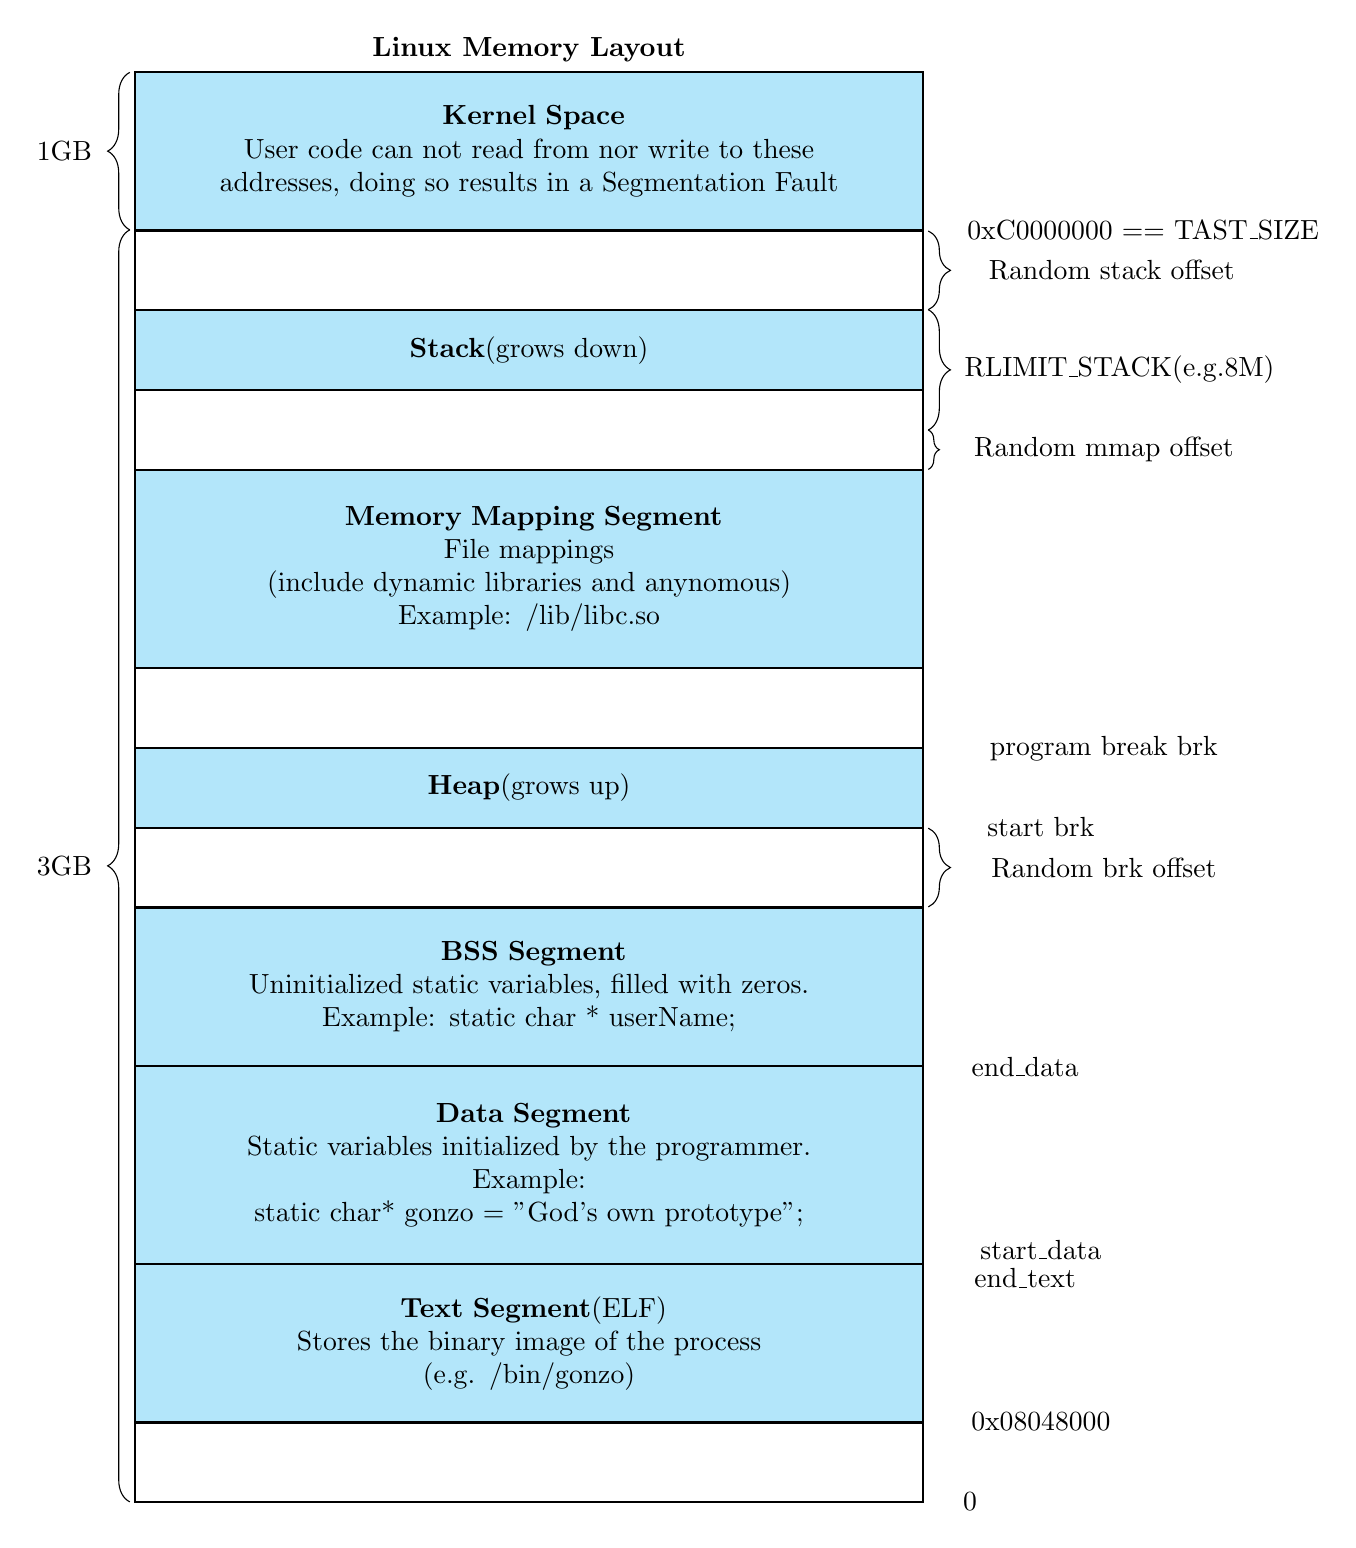
\begin{tikzpicture}
  [table/.style={
      draw,
      inner sep=0pt,
      matrix of nodes,
      nodes in empty cells,
      nodes={
        draw,
        align=center,
        text width=10cm,
        minimum width=10cm,
        outer sep=0pt,
        inner sep=0pt
      }
   },
   blank cell/.style={fill=white,minimum height=1cm},
   non blank cell/.style={fill=cyan!30,minimum height=#1}
  ]
   \matrix (layout) [table,label={[align=center]90:{\bf Linux Memory Layout}}]
   {
     |[non blank cell=2cm](kernel space)| {
        \textbf{Kernel Space}\\
        User code can not read from nor write to these\\
        addresses, doing so results in a Segmentation Fault}\\ % kernel space
     |[blank cell](stack offset)|{}\\ % random stack offset
     |[non blank cell=1cm]|{\textbf{Stack}(grows down)}\\ % stack
     |[blank cell](mmap offset)|{}\\ % random mmap offset
     |[non blank cell=2.5cm]|{
        \textbf{Memory Mapping Segment}\\
        File mappings\\
        (include dynamic libraries and anynomous)\\
        Example: /lib/libc.so}\\ % memory mapping segment
     |[blank cell]|{}\\ % 
     |[non blank cell=1cm](heap)|{\textbf{Heap}(grows up)}\\ % heap
     |[blank cell](brk offset)|{}\\ % random brk offset
     |[non blank cell=2cm](bss)|{
        \textbf{BSS Segment}\\
        Uninitialized static variables, filled with zeros.\\
        Example: static char * userName;}\\ % bss
     |[non blank cell=2.5cm](data)|{
        \textbf{Data Segment}\\
        Static variables initialized by the programmer.\\
        Example: \\
        static char* gonzo = "God's own prototype";}\\ % data segment
     |[non blank cell=2cm](text)|{
        \textbf{Text Segment}(ELF)\\
        Stores the binary image of the process\\
        (e.g. /bin/gonzo)}\\ % text segment
     |[blank cell](user space)|{}\\
   };
   % comments
   \draw [decorate,decoration={mirror,brace,amplitude=8pt,raise=2pt}]
      (kernel space.north west) -- (kernel space.south west) node[midway,xshift=-.9cm]{1GB};
   \draw [decorate,decoration={mirror,brace,amplitude=8pt,raise=2pt}]
      (kernel space.south west) -- (user space.south west) node[midway,xshift=-.9cm]{3GB};
   \node at ([xshift=2.8cm]kernel space.south east) {0xC0000000 == TAST\_SIZE};
   \draw [decorate,decoration={brace,amplitude=8pt,raise=2pt}]
      (stack offset.north east) -- (stack offset.south east) node[midway,xshift=2.4cm]{Random stack offset};
   \draw [decorate,decoration={brace,amplitude=8pt,raise=2pt}]
      (stack offset.south east) -- (mmap offset.east) node[midway,xshift=2.5cm]{RLIMIT\_STACK(e.g.8M)};
   \draw [decorate,decoration={brace,amplitude=4pt,raise=2pt}]
      (mmap offset.east) -- (mmap offset.south east) node[midway,xshift=2.3cm]{Random mmap offset};
   \node at ([xshift=2.3cm]heap.north east) {program break brk};
   \node at ([xshift=1.5cm]heap.south east) {start brk};
   \draw [decorate,decoration={brace,amplitude=8pt,raise=2pt}]
      (brk offset.north east) -- (brk offset.south east) node[midway,xshift=2.3cm]{Random brk offset};
   \node at ([xshift=1.3cm]data.north east) {end\_data};
   \node at ([xshift=1.5cm,yshift=.5em]data.south east) {start\_data};
   \node at ([xshift=1.3cm,yshift=-.5em]text.north east) {end\_text};
   \node at ([xshift=1.5cm]text.south east) {0x08048000};
   \node at ([xshift=.6cm]user space.south east) {0};
\end{tikzpicture}


  \section[Java命令行使用方法]{Java命令行使用方法}
  大家几乎都被IDE绑架了,谁还关注命令行java呢?\par
  注意:java的参数都是使用“-”的,不论长格式还是短格式,这跟GNU格式不符。
  \subsection[编译命令:javac]{编译命令:javac}
  \cmd{javac -classpath </path/to/folder;/path/to/.jar;/path/to/.zip>\\
        \hspace*{5em}-sourcepath </path/to/folder;/path/to/.jar;/path/to/.zip>}
  -classpath的值可以是folder、.jar、.zip,其中包含的都是.class文件;\\
  -sourcepath的值可以是folder、.jar、.zip,其中包含的都是.java文件。

  \subsection[运行命令:java]{运行命令:java}
  \cmd{javac -classpath </path/to/folder;/path/to/.jar;/path/to/.zip> runnable}
  -classpath的值可以是folder、.jar、.zip,其中包含的都是.class文件。\\
  runnable是一个.class文件,扩展名.class不要加上。

  \subsection[反汇编命令:javap]{反汇编命令:javap}
  javap是java的反汇编命令,但是很少有人用它来进行反汇编,
  原因是有很多其他工具反汇编工作做的比javap好的多,但是
  用javap来输出.class文件的字节码信息,对于学习JVM来说是
  很有帮助的。
  \cmd{javap -verbose runnable}
  注意:runnable为.class文件,后缀.class不要加上。

  \section[Windows客串:命令行模式启动Emacs]{Windows客串:命令行模式启动Emacs}
  直接在cmd中使用'emacs'启动时,cmd会一直被占用,使用'\&'也不行,可以使用
  'runemacs'代替'emacs',此为Emacs的命令行模式,cmd不会被占用。

  \section[常用压缩/解压缩命令]{常用压缩/解压缩命令}
  命令行下有很多压缩、解压缩命令,其中tar可以包含很多,另外还有就是zip、rar格式。
  \subsection[zip文件的压缩和解压缩]{zip文件的压缩和解压缩}
  压缩:zip filename.zip dirname\\
  解压:unzip filename.zip
  \subsection[rar文件的压缩和解压缩]{rar文件的压缩和解压缩}
  压缩:rar a filename.rar dirname\\
  解压:rar x filename.rar
  \subsection[使用tar处理不同的压缩和解压缩文件]{使用tar处理不同的压缩和解压缩文件}
  tar的基本使用格式如下:
  压缩:tar <algorithm>cvf filename.tar.<postfix> dirname\\
  解压:tar <algorithm>xvf filename.tar.<postfix>\\
  其中,v表示verbose,f表示file,而各种压缩算法及其对应的后缀如下所示:\par
  \begin{center}
  \begin{tabular}{ccc}
    \hline
    算法 & 字母表示 & 后缀\\ \hline
    gzip & z & .gz\\
    bzip & j & .bz\\
    bzip2 & j & .bz2\\
    compress & Z & Z\\ \hline
  \end{tabular}
  \end{center}
  如采用gzip算法的压缩和解压:\\
  压缩:tar zcvf filename.tar.gz dirname\\
  解压:tar zxvf filename.tar.gz


  \section[curl命令示例]{curl命令示例}
  使用curl命令获取外部IP地址:
  \cmd{curl ifconfig.me}
  注意:Window版本的curl也可以使用该命令!


  \section[树形结构显示文件夹内容]{树形结构显示文件夹内容}
  Windows版本:
  \cmd{tree /F}

  Linux版本:待添加。。。


  \section[pstree显示进程数结构]{pstree显示进程数结构}
  命令如下:
  \cmd{pstree -a -h}
  -a: 显示命令的启动参数\\
  -h: 高亮当前进程


  \section[login and interactive shell]{login and interactive shell}
  bash分为两种启动方式:\\
  Login shell 和 Interactive shell

  Interactive shell(交互式shell)很好理解,就是执行完一条命令就等待用户
  的下一条命令,以此完成跟用户之间的交互;Non-interactive shell,即
  非交互式shell,这种shell启动起来是为了执行bash script文件,它直接
  执行文件,而不跟用户进行交互,执行完脚本文件即退出。

  交互式shell通过"-i"选项启动,启动之后PS1被设置。

  判断shell是否为交互式shell的方法:\\
  echo \$-\\
  如果输出中包括''i''表示为交互式的,否则为非交互式的。

  Login shell通过''--login''选项启动,它要求用户输入账号信息进行登录,
  如纯文本方式登录系统,此时需要用户认证,而通过GUI登录系统之后,再次
  启动shell时是无需再次认证的(GUI登录时已经认证过了),此时就可以启动
  Non-login shell。

  登录式shell与非登录式shell最值得关注的是配置文件的加载,通常情况下加载
  顺序是这样的:\\
  Login shell:\\
  登录时:\\
  if /etc/profile exists, source it.
  
  if \~{}/.bash\_profile exists, source it.\\
  else if \~{}/.bash\_login exists, source it.\\
  else if \~{}/.profile exists, source it

  退出时:\\
  if \~{}/.bash\_logout exits, source it.

  一般会在这些配置文件中source其他配置文件,如profile文件中就经常会把
  .bashrc文件source进来。

  Non-login shell:\\
  登录时:\\
  if \~{}/.bashrc exists, source it.

  登录式shell与非登录式shell的退出方式也有些差异:\\
  exit 既可以退出login shell也可以退出non-login shell\\
  logout 只能退出login shell,退出non-login shell时会提示并建议用exit退出。

  另外,如果bash是通过sh启动的话,它会尽可能的模拟sh的行为,对于Login shell
  只会source /etc/profile和\~{}/.profile,其他配置文件将会被忽略。


  \section[统计整个目录里的文件行数]{统计整个目录里的文件行数}
  1. cat `find . -type f -print` | wc -l\\
  2. find . -type f -print | xargs cat | wc -l\\


\end{document}
